\documentclass[a4paper,11pt,danish,oneside]{article}

\usepackage[utf8]{inputenc}

\usepackage[danish]{babel}

\usepackage{graphicx}

\usepackage{multicol}

\usepackage[T1]{fontenc}

\usepackage[top=3cm, bottom=3cm, left=2.5cm, right=3.5cm]{geometry}

\usepackage{tocvsec2}

\usepackage{float}

\usepackage{tabularx}

\usepackage{parskip}

\usepackage{mathtools}

\usepackage{changepage}

\usepackage{mdwlist}

\usepackage{algorithm}

\usepackage{titlesec}

\usepackage{algpseudocode}

\algrenewcommand\algorithmicprocedure{\textbf{function}}

\usepackage[nottoc,numbib]{tocbibind}

\usepackage{setspace}

\linespread{1.4}

\titlespacing*{\section}{0pt}{0.5cm}{0cm}
\titlespacing*{\subsection}{0pt}{0.3cm}{0cm}
\titlespacing*{\subsubsection}{0pt}{0.1cm}{0cm}
\titlespacing*{\paragraph}{0pt}{0cm}{0cm}

\graphicspath{ {./Billeder/} }
\DeclareGraphicsExtensions{.pdf,.png,.jpg}
\begin{document}

\section*{Section}

\subsection*{Subsection}

\subsubsection*{subsubsection}

\section{Section}

\subsection{Subsection}

\subsubsection{subsubsection}

{\setstretch{1}
\begin{itemize}
	\item Første
	\item Anden
	\item Tredje
\end{itemize}
}

{\setstretch{1}
	\begin{enumerate}
		\item Første
		\item Anden
		\item Tredje
	\end{enumerate}
}

\begin{description}
	\setstretch{1}
	\item [Første]\hfill \\  beskrivelse 
	\item [Anden]\hfill \\  beskrivelse
	\item [Tredje]\hfill \\ beskrivelse
\end{description}

\begin{description}
	\setstretch{1}
	\item [Første] -  beskrivelse 
	\item [Anden] -  beskrivelse
	\item [Tredje] - beskrivelse
\end{description}

\begin{equation}
	s(n)=x(n)+2 \cos(2 \pi f) s(n-1)-s(n-2)
\end{equation}

Her er en ligning $s(n)=x(n)+2 \cos(2 \pi f) s(n-1)-s(n-2)$ den er i en tekst

\begin{table}[h]
	\begin{tabularx}{\textwidth}{|X|X|X|X|}
		\hline
		\multicolumn{2}{|l|}{\textbf{Goertzel}} & \multicolumn{2}{l|}{\textbf{FFT}} \\ \hline
	\textbf{Fordele} & \textbf{Ulemper} & \textbf{Fordele} & \textbf{Ulemper} \\ \hline
	Første & Anden & Tredje & Fjerde \\ \hline
	& & & \\ \hline
	\end{tabularx}
	\caption{Dette er en tabel}
	\label{tabel1}
\end{table}

nu referere jeg til tabel \ref{tabel1}

\begin{figure}[h]
	\centering
	
\includegraphics[scale=0.2]{1}
	\caption{1 i ovenstående linje, er navnet på billedet uden filendelse}
	\label{abelars}
\end{figure}

billede \ref{abelars} har labelet abelars


\begin{figure}[H]
	\centering
	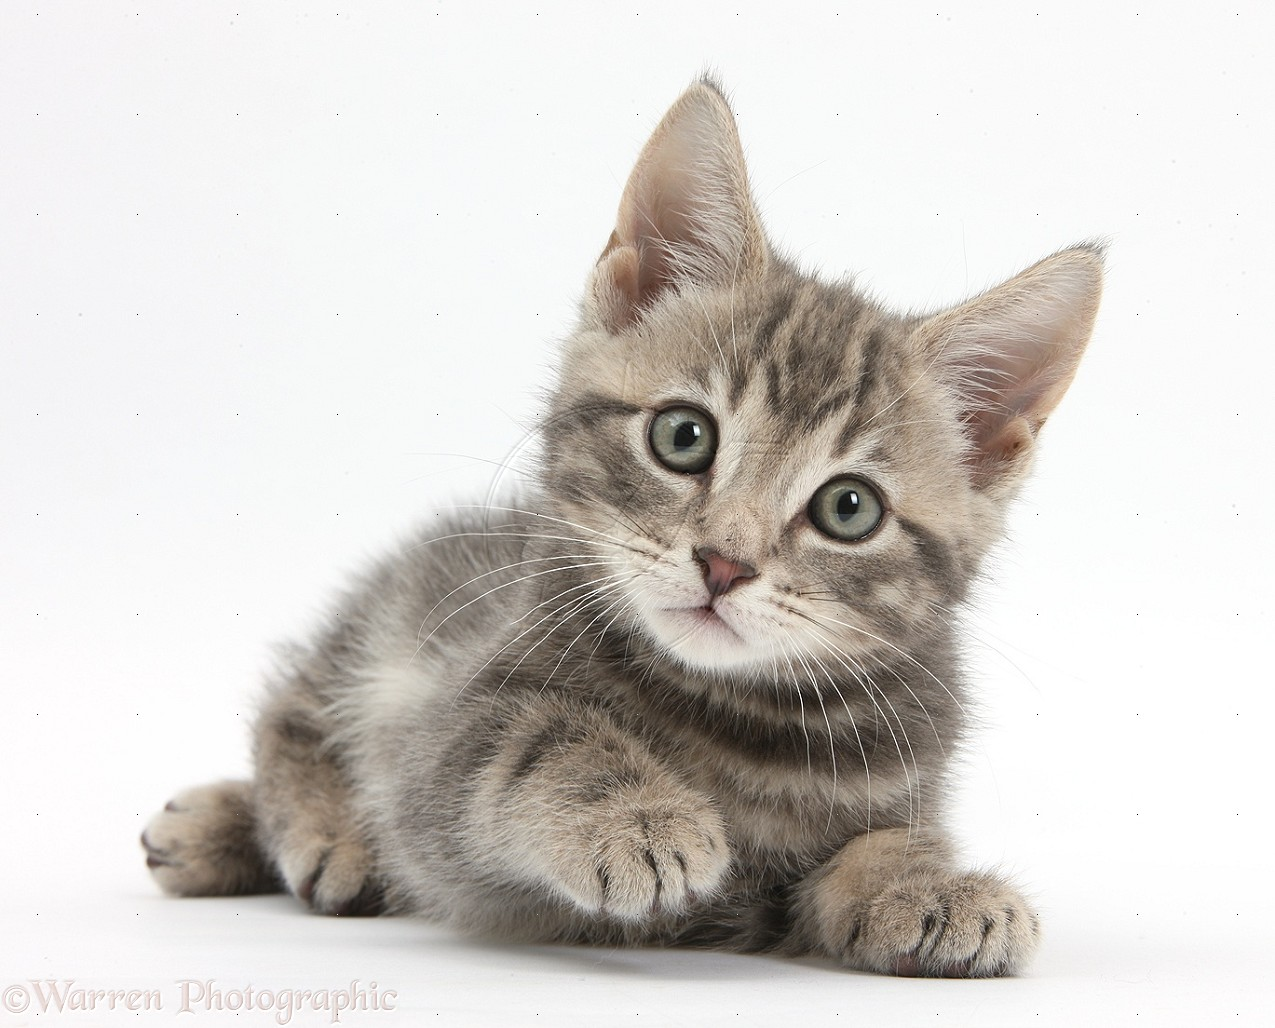
\includegraphics[scale=0.2]{2}
	\caption{Placering af billedet kan vælges efter  begin\{figure\} H er præcis her, h er cirka her, t er top, b er bund}
\end{figure}



\begin{algorithm}[h]
	\begin{algorithmic}[1]
		\Procedure{CRCencoder}{dataword}
		\State dividend = dataword
		\For{i from 0 to length of divisor - 1}
		\State append dividend with 0 
		\EndFor
		\For{i from 0 to length of dataword}
		\If{i'th element of dividend is 0}
		\For{j from 0 to length of divisor}
		\State set dividend i + j to dividend i + j \textbf{xor} with divisor j
		\EndFor
		\EndIf
		\EndFor
		\For{i from 0 to length of divisor - 1}
		\State append dataword with dividend i + length of dataword
		\EndFor
		\EndProcedure
	\end{algorithmic}
	\caption{Genererer redundante bit ud fra data.}
	\label{algo1}
\end{algorithm}

labels skal generelt bare benyttes over det hel. her refereres til algoritme \ref{algo1}

\begin{algorithm}[h]
	\caption{Forsøger at sende en pakke indtil der ankommer en ACK}
	\begin{algorithmic}[1]
		\Procedure{sendPacket}{}
		\While{packet not acknowledged}
		\If{packet has been sent 5 times unsuccessfully}
		\State connectionRelease()
		\State Break
		\EndIf
		\State send packet
		\State start timer
		\State wait until packet acknowledged or packet timed out
		\EndWhile
		\EndProcedure
	\end{algorithmic}
\end{algorithm}


\begin{figure}[h]
	\begin{center}
		\begin{minipage}{0.45\textwidth}
			\centering
			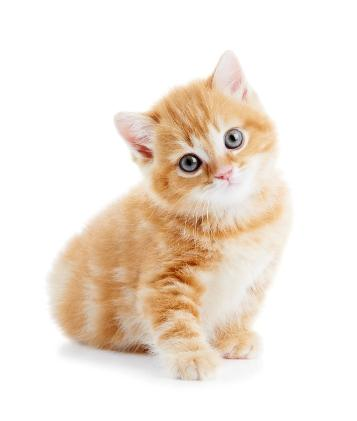
\includegraphics[scale=0.5]{3}
		\end{minipage}
		\begin{minipage}{0.45\textwidth}
			\centering
			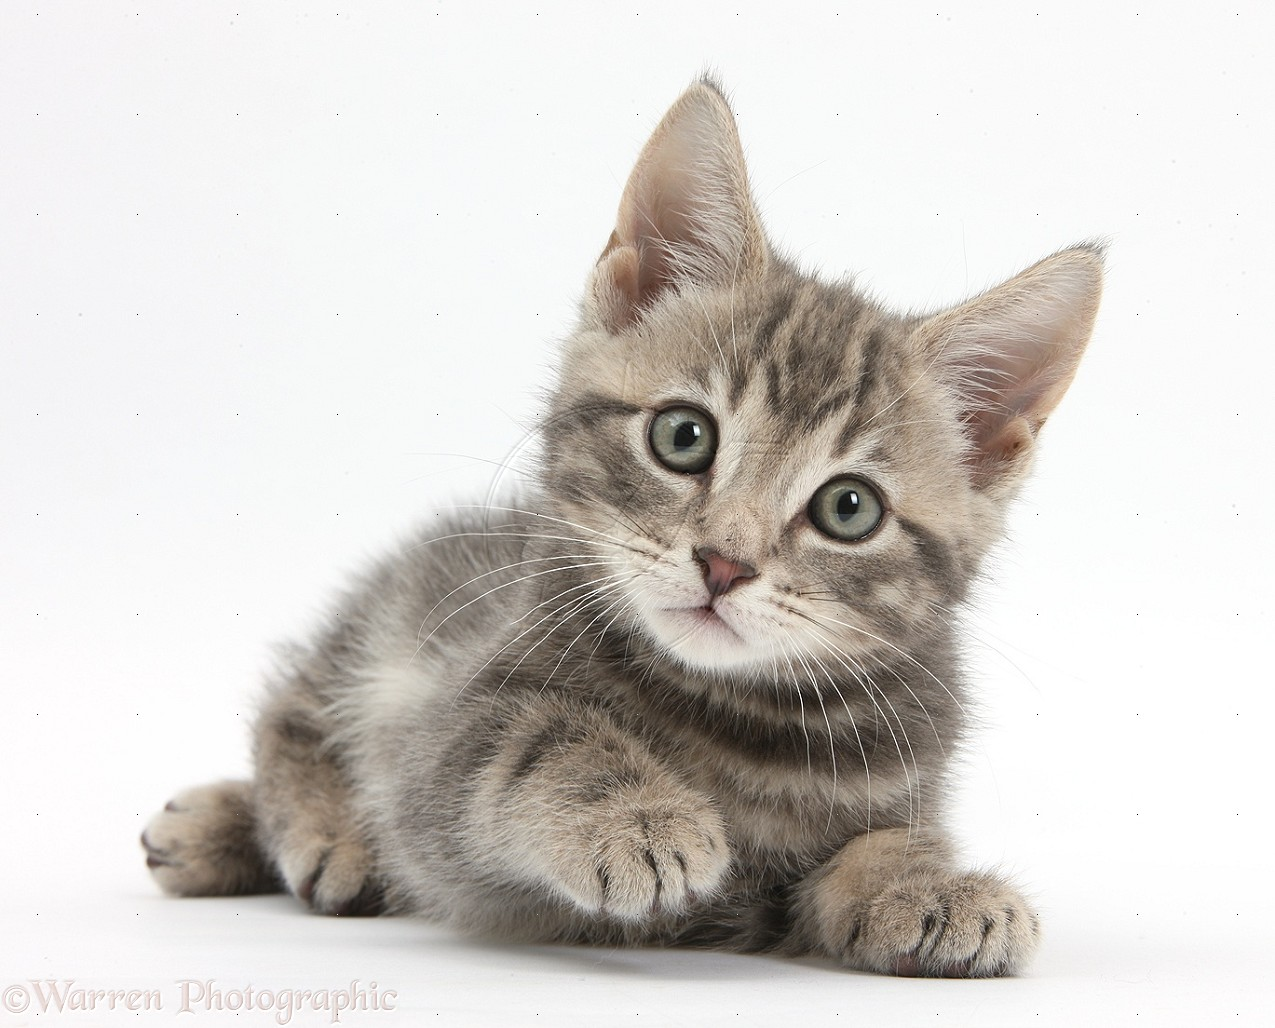
\includegraphics[scale=0.2]{2}
		\end{minipage}
		\caption{Her ses to billeder side om side, med en billedetekst}
	\end{center}
\end{figure}

\end{document}
